\documentclass{article}
\usepackage{graphicx}
%\textwidth=400pt
\usepackage{caption}
\captionsetup[table]{skip=10pt}
\usepackage{float}
\usepackage{longtable}
\usepackage[textwidth=14cm]{geometry}


\begin{document}

\begin{titlepage}

	\vfill
	
	\centering
	{\scshape\LARGE EUROPEAN BLOCKCHAIN ASSOCIATION \par}
	\vspace{1cm}
	{\huge\bfseries GOVERNANCE PROCESS \par}
	\vspace{2cm}
	
	\vfill
	Publication Date:\par
	\today

	\vfill
	
\end{titlepage}

\tableofcontents
\newpage

\section{EUROPEAN BLOCKCHAIN ASSOCIATION GOVERNANCE PROCESS}

\subsection{Preamble}

The EBA Governance Process is a set of binding rules, aiming at organizing the Association's governance and working procedures. 
Should there be any conflict between this EBA Governance Process and the EBA Bylaws, the Governance Process shall be subordinate to the regulations set forth in the Bylaws.

\subsection{Objective}

The European Blockchain Association e.V. (EBA) combines, synchronizes and leverages blockchain-related activities of European corporations, startups, venture capitalists, and scientific institutes. 
The EBA serves as a superior, neutral body to aggregate and coordinate blockchain activities throughout Europe and to provide Non-European parties with a direct API into the European blockchain ecosystem.

\subsection{DSAO Structure}

The EBA is a Decentralised Semi Autonomous Organisation (DSAO). 
A DSAO is a derivative of the original Decentralised Autonomous Organisation which describes a type of network connecting individual nodes that act autonomously on the basis of self-created rules. 
A DAO's financial transaction record and program rules are maintained on a blockchain and Member activities are not influenced by a central government.

Key differentiators between the EBA’s DSAO structure and a traditional DAO's:

\begin{itemize}
	\item {The EBA was founded as a legal entity - the European Blockchain Association e.V. - an association registered in Germany,}
	\item {The EBA is supported by a set of governance processes and is headed by the EBA Board of Directors. This facilitates the integration of the EBA into society at large. 
	It  addresses social, legal, economic and environmental aspects  as well as providing a point of contact for doing business. With this structure of a DSAO, the EBA combines the advantages of decentralised networks with the essential requirements of our society.}
\end{itemize}

\subsection{Core Elements of the DSAO}

The EBA consists of several entities which make up DSAO structure. Amongst these entities, but not limited to the entities listed, are the following:

\subsubsection{EBA Board of Directors}

The EBA is represented by the Board of Directors in and out of court. 
The Board represents the EBA to the outside world and decides on the principles of the work of the association, taking into account its objectives. The Board is elected by the General Meeting for a term of five years. 
The Board elected at the founding meeting is elected for the same duration. 
Re-election is permitted. 
Until a new election, the Board remains in office. 
The Board of Directors decides on the distribution of all financial resources and assets available to the association.

The Board manages the affairs of the association and directs all administrative tasks including:

\begin{itemize}
	\item {Preparation and implementation of the events of the association, the publication of its information resources and communications.}
	\item {Conclusion of leases for premises etc.}
	\item {Convocation and preparation of the General Meeting; the direction of the General Meeting.}
	\item {Accounting, preparation of the annual report and the fulfillment of related statutory and regulatory obligations.}
	\item {Issuing of orders as well as the conclusion and the termination of labor, works and other contracts, which are concluded with third parties to assist in the fulfillment of the statutory duties of the association.}
	\item {Admission and participation in the exclusion of Members}
\end{itemize}

The EBA Board of Directors may amend the EBA Governance Process as laid out in this document. 
These amendments shall be published within three business days prominently on the relevant EBA website.
Any full Member of the EBA may appeal to such modifications. 
Appeals are arbitrated by the Blockchain Arbitration Forum (BAF) (see section ‘Blockchain Arbitration Forum’, as well as ‘Checks and Balances’ in this document). 
Full Members of the EBA may also propose modifications to the EBA Governance Process. 
The Board of Directors is not, however, required to act upon such proposals.

\subsubsection{Working Groups}

The European Blockchain Association’s (EBA) Working Groups (hereafter: ‘WGs’) are established to facilitate the collaboration between the European Blockchain Association’s full Members. 
WGs are industry task forces that focus on building domain-specific blockchain PoCs and co-creating respective standards. 
Working Groups can steer the direction of blockchain related standards, protocols and industry norms across Europe. 
Working Groups play a special role within the EBA’s DSAO. 
As such there are a number of checks and balances on their activities as outlined within the EBA governance processes (see 'Working Group Process' section). 

\subsubsection{Extra Working Group Entities}

Extra-Working-Group-Entities are agile, mostly self-governing groups within the EBA. 
Any interested individual or institution may participate in such Extra-Working-Group-Entities. 
Participants can also be individuals or entities external to the EBA. 
This is explicitly wished in the case of public events organized by the EBA or its Extra-Working-Group-Entities.

Extra-Working-Group-Entities can be, but are not limited to:

\begin{itemize}
	\item {Local Blockchain Hubs: Local Chapters Throughout Europe}
	\item {Virtual Blockchain Hubs: EBA Website \& Communication Channels}
	\item {Academy: Educational Programs \& Scientific Research}
	\item {Events: Conferences, Hackathons, Meetups}
\end{itemize}

\subsubsection{Blockchain Arbitration Forum (BAF)}

The Blockchain Arbitration Forum (BAF) is the appellate body of the EBA. The BAF provides a venue for Members to appeal decisions made by the Board of Directors. 
In such cases, the BAF can make binding decisions overruling the board.

\subsection{Checks and Balances}

Figure \ref{C_B_Diagram} describes the process of checks and balances and appeals within the EBA. \\

\begin{figure}[h!]
  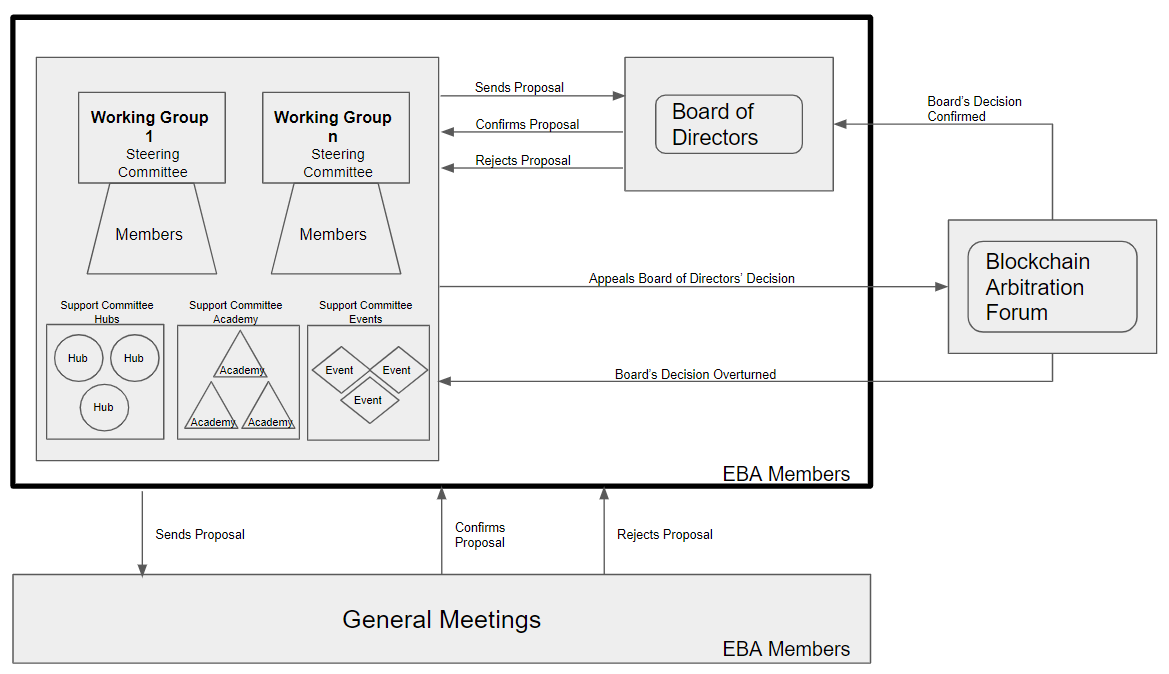
\includegraphics[width=\textwidth]{images/Governance_Checks_and_Balances.png}
  \caption{The EBA Checks and Balances}
  \label{C_B_Diagram}
\end{figure}

The Blockchain Arbitration Forum (BAF) is the appellate body of the EBA. The BAF provides a venue for Members to appeal decisions made by the  Board of Directors. 
In such cases, the BAF can make binding decisions overruling the Board. \\
If a proposal is rejected by the EBA Board of Directors, the entity whose proposal was rejected has the right of appeal. 
The Blockchain Arbitration Forum will base its decision on the spirit of the EBA code of conduct and governance guidelines as set forth in this document. \\
If the BAF rejects the appeal, the draft may be revised and resubmitted to the Board of Directors. 
If however, the BAF accepts the appeal, the Board of Directors must confirm the proposal.

\subsection{Ethical Code of Conduct}

\subsubsection{Preamble}

The EBA was founded to combine, synchronize and leverage blockchain-related activities of European corporations, startups, venture capitalists, and scientific institutes. \\
This Code of Conduct includes a set of principles and values that reflect the beliefs of EBA participants and their expectations towards their counterparties. \\
The EBA Code of Conduct is based on international conventions such as the Universal Declaration of Human Rights, the Guiding Principles on Children and Entrepreneurship, United Nations Guiding Principles on Business and Human Rights, the OECD Guidelines, and the UN Global Compact (Sustainable Development Goals). \\
Members of the EBA accept its Ethical Code of Conduct, and are obliged to adhere to the principles set out in this document. 
The EBA Members engage in a constructive and open dialogue with their business partners and stakeholders to pursue the principles of ethically responsible economic activity.
EBA Members not adhering to this Ethical Code of Conduct may have their Membership in the association terminated following a vote by the board of directors as outlined in the EBA Membership rules.

\subsubsection{Interpretation}

The EBA Code of Conduct covers all EBA Members as well as their business partners. \\
The EBA Governance Process and the EBA Bylaws are an integral part of the EBA Code of Conduct. The EBA Code of Conduct should be read and interpreted in conjunction with them.

\subsection{Our Values}

By adopting the EBA Code of Conduct and implementing it in their work, EBA Members are guided by the following values: \\

\textbf{Pursuit of Sustainable Development Goals SDGs} \\

The Sustainable Development Goals are inclusive, climate change, environmental degradation, prosperity, peace and justice. 
The Goals connect and in order to leave no one behind, it's important that we achieve each goal and target by 2030. \\

\textbf{Decentralized Semi-Autonomous Organization DSAO with Basic Governance} \\

The EBA's decentralized architecture allows autonomous individual activities of its Members. 
To facilitate the integration of the EBA in society with its social, legal, economic and environmental aspects, the EBA maintains a governance model. \\

\textbf{Member Economic Participation Grounded in a Blockchain Based Protocol} \\

At the heart of the EBA's architecture read a blockchain-based incentive scheme that motivates Members to actively participate in the DSAO. 
The crypto currency XSC can be used as a means to transfer value for all activities with the DSAO. \\

\textbf{Education, Access to and Sharing of Information} \\

The foundation of EBA's activities is laid out in the domain of blockchain and Distributed Ledger technologies, built by Individuals, companies, organizations and research institutes. \\

\textbf{Connecting the Dots: Synchronization of Member Activities} \\

The EBA's DSAO architecture integrates the aggregation and synchronization of blockchain and distributed ledger technology member activities in order to minimize inefficiently encapsulated and siloed developments. \\

\subsubsection{Implementation}

The principles set out in the EBA Code of Conduct establish the objectives and minimum expectations of EBA Members with regard to social behavior within the EBA.
While it is not possible to ensure full compliance with the Code by all their business partners at all times, EBA Members undertake to take appropriate measures to comply with the principles of the EBA Code of Conduct. \\
Compliance with national legislation is the first duty of the Members. 
In countries where national laws and regulations conflict with the EBA Code of Conduct, EBA Members should seek ways of complying with those principles that best meet EBA principles.

\subsubsection{Principles for Member Conduct}

The EBA expects all Members and business partners to comply with the EBA Code of Conduct insofar as this is possible under local law. \\

\textbf{No Discrimination} \\

EBA Members are prohibited from identifying individuals on the basis of gender, age, religion, race, caste, birth, social background, disability, ethnic or national origin, nationality, membership of workers' organizations, including trade unions, political membership or beliefs, sexual orientation, family responsibilities, civil status or any other situation that could lead to discrimination, exclusion or preference. 
In particular, Members may not be subject to harassment or disciplinary measures for the reasons stated above. \\

\textbf{Reasonable Remuneration} \\

EBA Members shall comply with these principles if, without prejudice to the specific expectations set out in this Agreement, they respect workers' right to adequate remuneration sufficient to enable them and their families to live decently and social benefits provided by law. \\
EBA Members are required to meet at least the legal minimum wage or, if higher, the industry standards approved on the basis of collective bargaining. \\
The wages are payable on time, regularly and completely in a legal tender. 
A partial payment in kind is permitted in accordance with the limits and requirements set out by local regulations. 
The level of wages has to reflect the qualifications and educational level of the employees and refers to the regular working hours. \\

\textbf{No Child Labor} \\

EBA Members comply with this principle if they do not, directly or indirectly, employ children under the legal age of compulsory school attendance, which may not be less than 15 years. 
This principle is intended to protect children from any form of exploitation in connection with EBA activities. \\

\textbf{No Forced Labor} \\

EBA Members may not resort to any form of servitude, forced or compulsory labor, serfdom, human trafficking or involuntary labor to directly or indirectly support EBA operations. \\

\textbf{Environmental Protection} \\

EBA Members shall comply with this principle if, without prejudice to the specific expectations set out in this code of conduct, they take the necessary measures to prevent environmental damage resulting from their activities within the EBA. \\

\textbf{Ethical Business} \\

EBA Members shall comply with this principle if, without prejudice to the objectives and expectations set out in this chapter, they are not involved in any form of bribery, blackmail, embezzlement or any form of bribery, including, but not limited to, the promise, offer or grant of any unfair financial or other incentives.\\
EBA Members are expected to have accurate information about their activities, structure and performance and to disclose it in accordance with applicable regulations and industry benchmarking practices especially with regard to EBA matters. \\
Furthermore EBA Members should additionally adhere to the EBA Antitrust Compliance Policy. \\

\textbf{Data Protection} \\

EBA Members must take reasonable care regarding the collection, storage and use of personally identifiable information (including the data of employees, business partners, customers, and consumers within their sphere of influence). 
Specifically, where required Members should adhere to industry best practices for GDPR compliance for all EBA business. 
Furthermore EBA Members should additionally adhere to the EBA Intellectual Property Rights Policy. \\

\textbf{Responsibility for Developed Software} \\

The EBA advises Members to take on a social constructivist point of view on technology. 
The Association is aware of the moral non-neutrality of technology: each technology has systematic effects on society, as it embodies a set of values, a framework and an ideology. 
Insofar, technologies are responsible for better or worse, since they are not merely tools people use for their own ends. 
Developers within the EBA will take this perspective into account when designing and implementing distributed ledger tools.

\newpage

\section{Membership Rules}

\subsection{Membership}

Members of the European Blockchain Association may be natural persons or legal entities (public or private law entities) as well as professorships and universities. 
Membership admission takes place after written application by the potential Member and by confirmation of the EBA Board of Directors. \\

Membership of the European Blockchain Association requires age of majority of natural persons.\\

The EBA's founding bylaws outline five basic types of Members:

\begin{enumerate}
	\item {Full Members with full voting rights} 
	\item Academic Members without voting rights
	\item Academic Members with full voting rights
	\item Honorary Members without voting rights
	\item Honorary Members with full voting rights
\end{enumerate}

These Membership types are further subdivided into a number of Membership subclasses as listed in Table \ref{table:Mem_Classes} on page \pageref{table:Mem_Classes}.

\subsection{Membership Classes}

\begin{longtable}{| p{.55\textwidth} | p{.45\textwidth} |}

	\hline
 	   \textbf{Membership Classes} & \textbf{Membership Fees per year, in Euros} \\ \hline\hline
 	   \textbf{1a) FULL MEMBERS w. Voting Rights - Legal entities (Startups, Corporations etc.)} &
	Startup: 2.500,- \newline Small: 15.000,- (\textless 50 staff) \newline Medium: 25.000,- (50 - 250 			staff)\newline Large: 50.000,- (\textgreater 250 staff)\newline Consulting Firms: 25.000,- \\
	\hline
		\textbf{1b) FULL MEMBERS w. Voting Rights Natural persons} & 2.500,- p.p. \\                                                                                                             	\hline
		\textbf{2a) FULL ACADEMIC MEMBERS w. Voting Rights - Legal entities (Universities, Professorships)} & 2.500,- p.p. \\                                                                                                             	\hline
		\textbf{2b) FULL ACADEMIC MEMBERS w. Voting Rights - Natural persons} & 2.500,- \\                                                                                                             	\hline
		\textbf{3a) HONORARY MEMBERS without Voting Rights - Legal entities} & No Membership Fees \\                                                                                                             	\hline
		\textbf{3b) 3b) HONORARY MEMBERS without Voting Rights Natural persons} & No Membership Fees \\                                                                                                             	\hline
	
	\caption{Membership Classes and the Corresponding Membership Fees}
	\label{table:Mem_Classes}

\end{longtable}

\textbf{1a) FULL MEMBERS w. Voting Rights - Legal entities (Startups, Corporations etc.)} \\

‘FULL MEMBERS w. Voting Rights - Legal entities’ shall be legal entities that agree to abide by the obligations set forth in the EBA Membership Rules, including, without limitation, the requirements set forth on Exhibit B of the EBA Membership Agreement. 
Legal entities as Full Members with Voting Rights shall be permitted to vote with the Membership At-Large, as set forth in the Bylaws. 
Legal entities as Full Members with Voting Rights are entitled to found Working Groups, and initially appoint their representatives to the Working Groups’ Steering Committee. 
Legal entities as Full Members with Voting Rights commit themselves to allocate at least one FTE to the activities of the EBA. 
‘FULL MEMBERS w. Voting Rights - Legal entities’ can be Member Participants of a Working Group (WG). These entities can participate and will have voting rights with respect to WG matters as outlined within each group's charter. 
This could include scheduling meetings and activities, access/participation in the development of all materials produced in the WG, Marketing Programs, Material development, mailing lists and wikis. \\

\textbf{1b) FULL MEMBERS w. Voting Rights - Natural persons} \\

‘FULL MEMBERS w. Voting Rights - Natural persons’ shall be individuals that agree to abide by the obligations set forth in the EBA Membership Rules, including, without limitation, the requirements set forth on Exhibit B of the EBA Membership Agreement. 
Full Members with Voting Rights as individuals shall be permitted to vote with the Membership At-Large, as set forth in the Bylaws. 
As Member Participants of a Working Group (WG), these individuals can participate and will have voting rights with respect to WG matters as outlined within each group's charter. 
This could include scheduling meetings and activities, access/participation in the development of all materials produced in the WG, Marketing Programs, Material development, mailing lists and wikis. \\

\textbf{2a) FULL ACADEMIC MEMBERS w. Voting Rights - Legal entities (Universities, Professorships etc.)}

‘FULL ACADEMIC MEMBERS w. Voting Rights - Legal entities’ shall be legal entities that agree to abide by the obligations set forth in the EBA Membership Rules, including, without limitation, the requirements set forth on Exhibit B of the EBA Membership Agreement. 
Legal entities as Full Academic Members with Voting Rights shall be permitted to vote with the Membership At-Large, as set forth in the Bylaws. Legal entities as Full Academic Members with Voting Rights are entitled to found Working Groups, and initially appoint their representatives to the Working Groups’ Steering Committee. 
Full Academic Members w. Voting Rights - Legal entities’ can be Member Participants of a Working Group (WG). These entities can participate and will have voting rights with respect to WG matters as outlined within each group's charter. 
This could include scheduling meetings and activities, access/participation in the development of all materials produced in the WG, Marketing Programs, Material development, mailing lists and wikis. \\

\textbf{2b) FULL ACADEMIC MEMBERS w. Voting Rights - Natural persons} \\

‘FULL ACADEMIC MEMBERS w. Voting Rights - Natural persons’ shall be individuals that agree to abide by the obligations set forth in the EBA Membership Rules, including, without limitation, the requirements set forth on Exhibit B of the EBA Membership Agreement. 
Full Academic Members with Voting Rights shall be permitted to vote with the Membership At-Large, as set forth in the Bylaws. 
As Member Participants of a Working Group (WG), these individuals can participate and will have voting rights with respect to WG matters as outlined within each group's charter. 
This could include including scheduling meetings and activities, access/participation in the development of all materials produced in the WG, Marketing Programs, Material development, mailing lists and wikis. \\

\textbf{3a) HONORARY MEMBERS without Voting Rights - Legal entities} \\

‘HONORARY MEMBERS without Voting Rights - Legal entities’ shall be legal entities that agree to abide by the obligations set forth in the EBA Membership Rules, including, without limitation, the requirements set forth on Exhibit B of the EBA Membership Agreement. 
Legal entities as Honorary Members without Voting Rights shall not be permitted to vote with the Membership At-Large. 
Honorary Members without Voting Rights are not permitted to join any Working Groups. \\

\textbf{3b) HONORARY MEMBERS without Voting Rights - Natural persons} \\

‘HONORARY MEMBERS without Voting Rights - Natural persons’ shall be individuals that agree to abide by the obligations set forth in the EBA Membership Rules, including, without limitation, the requirements set forth on Exhibit B of the EBA Membership Agreement. 
Individuals as Honorary  Members without Voting Rights shall not be permitted to vote with the Membership At-Large. Individuals as Honorary Members without Voting Rights are not permitted to join any Working Groups. They may however, be invited to sit in on meetings at the discretion of the Working Group. \\

Membership is not transferable. 
The exercise of Membership rights can not be left to another person. Legal entities, professorships, universities and corporations must name the natural person who will be able to exercise the rights of Membership in the Membership application. \\ 

The application for Membership must be submitted in writing, by signing the EBA Membership Agreement. The EBA Board of Directors decides on the admission of new Members. There is no entitlement to Membership. \\

In case prospective Members aiming to join the EBA, bring in sufficient in-kind contributions, the EBA Board of Directors can discount the Membership fee or waive the fee as appropriate, based on the in-kind contribution of the prospective Members.

\subsection{Rights and Obligation of Members}

\subsubsection{General Rights \& Obligations of Members}

All members must execute a Membership Agreement and pay the fees called thereon. 
Once accepted, Members shall be entitled to all rights and bound to all obligations generally afforded and imposed upon all Members of the European Blockchain Association. 
In addition, some Members shall be granted additional rights and obligations as a result of their participation in a Working Groups. \\

All Members pay Membership fees whose amount and due date are determined by the contribution regulations. 
For the year 2019 the defined contribution regulations apply. 
For the subsequent years, the Membership fee is decided by the general assembly on the proposal of the Board of Directors for the following financial year.  \\

\noindent {\bfseries Official Bank Account of the European Blockchain Association:\\}

\noindent The following bank details are to be used for all EBA official business including but not limited to the payment of membership fees:\\

\noindent {\bfseries Deutsche Skatbank\\}
Zweigniederlassung der\\
VR-Bank Altenburger Land eG\\
Altenburger Strasse 13\\
04626 Schmölln\\

\noindent {\bfseries IBAN\\}
DE94 8306 5408 0004 2278 60\\

\noindent {\bfseries BIC\\}
GENODEF1SLR\\

All Members are entitled to participate in the events, elections and votes of the European Blockchain Association, as well as the use of all other services under the statutory provisions. \\

This right is tied to the fulfillment of the contribution obligations.
Each Member is obliged to inform the European Blockchain Association about the change of the residential and registration address, email address, mobile and fixed telephone number as well as the name immediately and unsolicited in writing. 
Costs incurred by the European Blockchain Association for such investigations must be reimbursed by the Member. 
The costs of legal action for the (judicial) assertion of claims against a Member, which may be incurred by the European Blockchain Association, are also to be reimbursed to the European Blockchain Association. \\

All EBA Members agree to abide by the rules of as set forth by the EBA Code of Conduct.

\subsubsection{Voting Rules}

The EBA aims to apply general, free, equal, secret and blockchained-based voting sessions within the entire Association. \\
Voting Sessions will be held digitally on a blockchain-based voting platform. 
The voting should be set up by the system administrators of the EBA and made accessible to respective Members of the EBA. 
The set-up of the voting platform defines attributes like the options to vote on, the start and the end of the voting and the distribution of an individual link for a voting. 
Every Member that is eligible to vote, depending on its Membership class and/or Working Group affiliation will get an individual access code over the contact details provided which they have to enter when accessing the voting page. \\
This voting mechanism should be used within Working Groups, Working Groups Steering Committees, the Board of Directors, the Blockchain Arbitration Forum as well as during the General Meetings to decide on relevant matters to be decided with respect to each sub-group of the EBA. \\
Membership of the EBA can entail Voting Rights, depending on the Membership Class. 
Membership is divided in two overall classes, there are ‘Members with Voting Rights’ and ‘Members without Voting Rights’. 
Member Participants of Working Groups may have additional Voting Rights on top of their basic Voting Rights in relation to the work carried out within the respective Working Group. 
Voting Rights for Member Participants of Working Groups may be defined by the Working Group’s Steering Committee within the Working Group Charter. \\
The General Meeting for all EBA-Members with Voting Rights has the purpose to discuss and decide on proposals for changes of organizational matters that are applicable for the whole EBA (i.e. changes to the bylaws, changes to the governance process). \\
For all Members with Voting Rights, whether legal entities or individuals, the principle of ‘one Member - one vote’ applies.

Any election, unless otherwise indicated in the EBA governance process, votes within the EBA will be decided by a simple majority. \\
The table \ref{table:Mem_Voting} on page \pageref{table:Mem_Voting} gives an overview over the Voting Rights per respective Membership class: \\

\begin{longtable}{| p{.30\textwidth} | p{.70\textwidth} |}

	\hline
    \textbf{Membership Classes} & \textbf{Voting Rights} \\ \hline\hline
    \textbf{1a) FULL MEMBERS w. Voting Rights  - Legal entities (Startups, Corporations etc.)} & 
    
   	\begin{itemize}
   		\item Propose and vote for Working Group Steering Committees
   		\item In case the Member is a Participant of a Working Group: Voting Rights with respect to WG matters as outlined within each group's charter (e.g. scheduling meetings and activities, access/participation in the development of all materials produced in the WG, Marketing Programs, Material development, mailing lists and wikis)
   		\item Vote on proposals for changes of organizational matters that are applicable for the whole EBA during the EBA General Meeting
   	\end{itemize}\\ \hline
    	
   	\textbf{1b) FULL MEMBERS w. Voting Rights - Natural persons} & 
   	\begin{itemize}
   		\item In case the Member is a Participant of a Working Group: Voting Rights with respect to WG matters as outlined within each group's charter (e.g. scheduling meetings and activities, access/participation in the development of all materials produced in the WG, Marketing Programs, Material development, mailing lists and wikis)
   		\item Vote on proposals for changes of organizational matters that are applicable for the whole EBA during the EBA General Meeting
   	\end{itemize}\\ \hline
    	
   	\textbf{2a) FULL ACADEMIC MEMBERS w. Voting Rights - Legal entities (Universities, Professorships etc.)} & 
   	\begin{itemize}
   		\item Propose and vote for Working Group Steering Committees
   		\item In case the Member is a Participant of a Working Group: Voting Rights with respect to WG matters as outlined within each group's charter, (e.g. scheduling meetings and activities, access/participation in the development of all materials produced in the WG, Marketing Programs, Material development, mailing lists and wikis)
   		\item Vote on proposals for changes of organizational matter that are applicable for the whole EBA during the EBA General Meeting
   	\end{itemize}\\ \hline
    	
   	\textbf{2b)FULL ACADEMIC MEMBERS w. Voting Rights - Natural persons} &
   	\begin{itemize}
   		\item In case the Member is a Participant of a Working Group: Voting Rights with respect to WG matters as outlined within each group's charter, (e.g. scheduling meetings and activities, access/participation in the development of all materials produced in the WG, Marketing Programs, Material development, mailing lists and wikis)
   		\item Vote on proposals for changes of organizational matter that are applicable for the whole EBA during the EBA General Meeting
   	\end{itemize}\\ \hline
    	
   	\textbf{3a) HONORARY MEMBERS without Voting Rights - Legal entities} &
   	\begin{itemize}
   		\item No Voting Rights
   	\end{itemize}\\ \hline
    	
   	\textbf{3b) HONORARY MEMBERS without Voting Rights - Natural persons} &
   	\begin{itemize}
   		\item No Voting Rights
   	\end{itemize}\\ \hline 
	    	
	\caption{Voting Rights of Membership Classes}
	\label{table:Mem_Voting}
\end{longtable}

\subsection{Late Fees, Costs and Expenses}

\subsubsection{Late Fees}

If a Member’s payment of its annual Membership dues is not fully paid within sixty (60) days of its invoice due date, a late fee representing one percent (1\%) of the delinquent Membership dues shall be added to such Membership dues, compounding monthly, commencing on the 31st day following invoice date. 
Additionally, if a Member qualifies for quarterly payment of its annual Membership dues (according to Exhibit B of the EBA Membership Agreement) and has not fully paid a payment within thirty (30) days of its invoice due date, a late fee representing one percent (1\%) of the delinquent Membership dues shall be added to such Membership dues, compounding monthly, commencing on the 31st day following invoice date.

\subsubsection{Costs and Expenses}

Each Member shall bear all of its own costs and expenses related to Membership in the European Blockchain Association including, but not limited to, compensation payable to Member’s employees and consultants that participate in the European Blockchain Association on behalf of Members, and all travel and other expenses associated with Member’s participation in European Blockchain Association meetings, conferences, and development projects. 
Except as otherwise set forth in these Membership Rules, the Membership Agreement, or in the Bylaws, Members understands and agrees that Members have no rights of reimbursement from the European Blockchain Association. 
Members and working groups may however petition the Board of Directors for funding milestone based grants derived from Membership dues for specific projects or expenses. 
The decision over how to allocate this funding is entirely up to the Board of Directors but such decisions may be appealed to the Blockchain Arbitration Forum.

\subsubsection{Compliance with Policies}

Members agree to abide by, and shall have all applicable rights and obligations as set forth in, the European Blockchain European Blockchain Association’s bylaws, the European Blockchain European Blockchain Association’s Intellectual Property Rights Policy (the “IPR Policy”), and all additional policies and procedures adopted by the European Blockchain Association, as may be amended from time to time in accordance with the European Blockchain Association’s bylaws.

\subsection{Compliance with Licences}

Members review, and agree to abide by, and shall have all rights and obligations as set forth in the European Blockchain Association’s Intellectual Property Rights Policy (IPR Policy), as may be amended from time to time in accordance with the EBA’s bylaws. 
Members agree to follow all licencing procedures as set forth in the European Blockchain Association’s Intellectual Property Rights Policy, unless otherwise agreed to in accordance with the EBA’s bylaws and IPR Policy.

\subsection{General Meeting}

The General Meeting takes place at least once a year at the invitation of the Board of Directors, but for the first time in the calendar year 2019. 
An extraordinary General Meeting shall be convened if the Board of Directors resolves the convocation for urgent and important reasons. 
All Members of the European Blockchain Association are entitled to participate in the General Meeting. \\
The General Meeting shall be called by the Board of Directors with a notification period of at least two weeks, including the General Meeting’s agenda. 
The deadline begins with the day following the dispatch of the letter of invitation or the invitation email. 
The letter of invitation shall be deemed to have been received by the Member if it has been addressed to the address last notified to the representative Board. 
As an invitation, sending an email to the last known email address of the Member is sufficient. \\

The General Meeting decides in particular:

\begin{enumerate}
	\item Election and discharge of the Board of Directors
	\item Determination of Membership fees and resolution of the contribution regulations
	\item Acceptance of the reports of the Board of Directors
	\item Resolution on motions to the General Meeting
	\item Resolution on amendments to the bylaws of the European Blockchain Association
	\item Dissolution of the European Blockchain Association	
\end{enumerate}

Each duly convened General Meeting has a quorum. All decisions are taken by a simple majority of the voting Members present. 
Amendments to the bylaws require a majority of three-quarters of those present, as well as decisions on the change of the purpose of the European Blockchain Association or the dissolution of the European Blockchain Association. 
They can only be taken if they have been previously announced in a written format to each of the Members. 
The proceeding of the General Meeting of the European Blockchain Association is to be documented in the official meeting minutes. 
A scribe will be responsible for ensure the accuracy of these minutes. \\
In principle, all elections and votes are aimed to be held by a blockchain based voting system. 
In case of a tie, both Directors have double voting rights. \\
The General Meeting elects the Members of the Board of Directors individually and with a simple majority of the Members present. 
If there is a tie, another ballot takes place. If there is a new tie, the tie will be broken by the drawing of lots.

\subsection{Delinquency: Non-payment of Fees}

In the event that a Member does not pay their annual Membership dues and all compounded late fees within ninety (90) days of the invoice due date (“Dues Delinquent”), the Membership of such Member shall, without further action by the Board of Directors or the Membership At-Large, be terminated.

\subsection{Termination of Membership}

The Membership of any Member shall terminate upon the occurrence of any one or more of the following: \\

\textbf{(a) Resignation} \\

Any Member may resign from the European Blockchain Association via a written request filed with a Member of the management Board. 
The resignation of a Member shall not relieve the Member from any payment obligations the Member may have to the European Blockchain Association as a result of obligations incurred or commitments made prior to resignation. 
Except as otherwise set forth in these Bylaws, a resigning Member shall not be entitled to receive any refund, pro rata or otherwise, of any Membership fee, dues or assessments for the balance of the calendar year in which the resignation is effective. 
Within ten (10) days of resigning from the European Blockchain Association , a Member may appeal in writing to the Board for a pro rata refund of its annual Membership dues. 
The appeal will specifically set forth any circumstances that the Member believes justify a refund in its case. 
The Board shall decide by simple majority upon the appeal in its sole discretion at its first meeting following the appeal scheduled under Section. \\

\textbf{(b) Expulsion, Termination or Suspension} \\

The Membership of any Member may be terminated “For Cause” upon the affirmative vote of two-thirds (2/3) of the Members of the Board after a hearing duly held in accordance with this Section. 
As used in this Section, here, a two-thirds (2/3) vote means two-thirds (2/3) of the Members of the Board exclusive of any director is who is facing expulsion or suspension (any such director, shall be referred to as the “Affected Director”).
 For purposes of this Section “For Cause” shall mean that the Member has materially breached the Membership Agreement, Code of Conduct, Bylaws, IPR Policy, Antitrust Policy and/or other related European Blockchain Association agreements or policies, and has not cured such breach within thirty (30) days of receipt of written notice from the European Blockchain Association.\\
Such determination shall be made in the sole and absolute discretion of the Board (excluding the Affected Director).
 Following the determination by the Board that a Member should be terminated the following procedures shall apply: \\
 
1. A notice shall be sent by mail by prepaid, first-class or certified mail to the most recent address of such Member as shown on the European Blockchain Association's records, setting forth the termination and the reasons therefore. Such notice shall be sent at least fifteen (15) days before the proposed effective date of the termination. \\

2. The Member being terminated shall be given an opportunity to be heard, either orally or in writing, at a hearing to be held no fewer than five (5) days before the effective date of the proposed termination. 
The hearing shall be held by the European Blockchain Association's Board. 
The notice to the Member of its proposed termination shall state that such Member is entitled, upon request, to such hearing, shall state that a date, time and place of the hearing will be established upon receipt of request therefore, and shall state, that in the absence of such request, the effective date of the proposed termination. \\

3. In the event that a hearing is held, then following such hearing the Board (excluding the Affected Director) shall decide whether such Member should in fact be terminated, or sanctioned via written reprimand as determined by the Board; provided, that, any such decision to terminate or sanction such Member must be approved by a vote of two-thirds (2/3) of the Board (excluding the Affected Director). 
The decision of the Board shall be final unless there is a successful appeal decision through the Blockchain Arbitration Forum. \\ 

4. Any action challenging a termination of Membership of a Member, including any claim alleging defective notice, must be commenced within fifteen (15) days after the date of the termination. \\

\textbf{(c) Reinstatement} \\

Members terminated pursuant to Section(b) may only be reinstated upon the affirmative vote of at least two-thirds (2/3) of the Directors in Good Standing represented at a Board meeting at which a quorum is present. \\

\textbf{(d) Non-Liability} \\

No Member shall be liable for the debts, liabilities, or obligations of the European Blockchain Association merely by reason of being a Member. \\

\textbf{(e) Assignment} \\

Upon the completion of any acquisition or merger involving a Member in which the Member is not the surviving entity, the Board, in its sole discretion, may permit such Member’s Membership to be transferred to the surviving entity.

\subsection{Press Releases}

A new member shall assist the European Blockchain Association in publicly announcing such new member’s Membership therein within ninety (90) days of joining the Association. 
A Member may make public announcements or press releases concerning its own activities as a member. 
Unless otherwise required by law, any press release concerning a Member made by the European Blockchain Association or another Member shall be subject to that member's prior written consent. 
Once approved, the press release statement may be used by the European Blockchain Association and other Members for the purpose of promoting the Association (or such purpose as is designated in the member's consent) and reused for such purpose until such approval is withdrawn with reasonable prior written notice. 
Any use of a Member's name shall be subject to the applicable usage guidelines of that Member.

\subsection{Data Processing Clause}

The Member agrees by joining the association that all personal data disclosed or become known within the framework of the Membership may be stored, processed and used by the European Blockchain Association exclusively in strict connection to the purpose of the European Blockchain Association. \\
Each Member agrees that the name, address, email address and telephone of Members as well as Members of tax advisory and legal professions, which are required to professional secrecy, may be disclosed and allow them to use the same, solely in the interest of orientation on the purpose of the European Blockchain Association to promote and support the implementation of the European Blockchain Association's goals.

\newpage

\section{Bylaws}

\subsection{\S 1 Name, Registered Office, Fiscal Year}

\begin{enumerate}
	\item The association bears the name 'EUROPEAN BLOCKCHAIN ASSOCIATION' (hereinafter referred to as 'association'). 
	He is to be registered in the association register. 
	After registration, he receives the suffix 'e.V.'.
	\item The club is based in Munich.
	\item Fiscal year is the calendar year.
\end{enumerate}

\subsection{\S 2 Purpose of the Association}

\begin{enumerate}
	\item The purpose of the association is the promotion of the exchange of opinions and experiences as well as the exploration of the potentials of Blockchain and Distributed Ledger Technologies (DLT).
	\item The purpose is achieved in particular by: \\
	
	\begin{itemize}
		\item Establishing contacts and networks in politics and administration - especially in Europe,
		\item Organizing and initiating events and conferences,
		\item Creation of knowledge bases for respective industry clusters,
		\item Networking of knowledge from research and teaching with membership and business,
		\item Creation of a virtual academy for know-how from the entire Blockchain or DLT area,
		\item Establishment of industry standards,
		\item Networking and matchmaking	
	\end{itemize}
	
	\item The association is selfless and non-partisan; he does not pursue primarily self-economic purposes. Funds of the association may only be used for statutory purposes. The members receive no profit shares and in their capacity as members also no other donations from means of the federation.
\end{enumerate}

\subsection{\S 3 Membership}

\begin{enumerate}
	\item Members of the Association may be natural or legal persons as well as professorships, universities and public or private law entities. The admission takes place after written application by the potential member and by confirmation of the executive committee.
	\item The membership of the association requires the natural age of the majority of the member.
	\item There are the following categories of members:
	
	\begin{enumerate}
		\item Full members with full voting rights
		\item  Academic members without voting rights
		\item  Academic members with full voting rights
		\item  Honorary members without voting rights
		\item  Honorary members with full voting rights
	\end{enumerate}
	
	\item Membership is not transferable. 
	The exercise of membership rights can not be left to another. 
	Legal persons, professorships, universities and corporations must name the natural person in the application for membership, who should be able to exercise the rights of membership.
	\item The application for membership must be submitted in writing. 
	The board decides on the admission of new members. 
	There is no entitlement to membership.
	\item Membership ends by resignation, expulsion, death (natural persons) or by dissolution (legal persons) of the member or termination of the liquidation and the subsequent deletion in the commercial register.
	\item Resignation from the association must be made in writing to a member of the management board and is possible in each case subject to a notice period of six months to the end of the calendar year.
	\item A member can only be excluded for good cause.
	 Important reasons are, in particular, conduct that harms the objectives of the association, violation of statutory obligations, the disclosure of information obtained by a member by the association to non-members (except third-party professional liability) or arrears of contributions due more than three months, The Executive Board decides on the exclusion. \\
The exclusion decision will be communicated to the member in writing by letter or e-mail to the last known address and will become effective with the dispatch. 
The member is entitled to appeal to the general meeting against the exclusion, which must be addressed in writing to the board within one month. 
The general meeting decides finally. The ordinary legal process is open against the decision.
	\item Upon termination of membership, there is no entitlement to a share of the association's assets.
\end{enumerate}

\subsection{\S 4 Organs of the Association}

Organs of the association are: \\
\begin{itemize}
	\item The General Meeting
	\item The Board
\end{itemize}

\subsection{\S 5 Rights and Obligations of the Members}

\begin{enumerate}
	\item All members pay membership fees whose amount and due date are determined by the contribution regulations. 
	For the year 2019 the defined contribution regulations apply. 
	For the subsequent years, the membership fee is decided by the general meeting on the proposal of the executive board for the following financial year.
	\item All members are entitled to participate in the events, elections and votes of the association, as well as the use of all other services under the statutory provisions. \\
This right is tied to the fulfillment of the contribution obligations. 

	\item Each member is obliged to inform the association about the change of the residential and registration address, e-mail address, mobile and fixed telephone number as well as the name immediately and unsolicited in writing. 
	Costs incurred by the Association for such investigations must be reimbursed by the Member. 
	The costs of legal action for the (judicial) assertion of claims against a member, which may be incurred by the association, are also to be reimbursed to the association.
\end{enumerate}

\subsection{\S 6 Board}

\begin{enumerate}
	\item The executive committee consists of three members, namely the chairman and two deputy directors. 
	The board has joint power of attorney. 
	He forms the board within the meaning of § 26 BGB. 
	The Executive Board, ie both the Executive Board and the Deputy Executive Board, are each consistently and at least exempted from the restrictions of § 181 BGB.
	\item The association is represented by the executive committee in and out of court. 
	He represents the club to the outside and decides on the principles of the work of the association, taking into account the purpose of the club.
	\item The Executive Board is elected by the General Assembly for a term of five years. 
	The board elected at the founding meeting is elected for the same duration. 
	Re-election is permitted. 
	Until a new election, the board remains in office.
	\item The board manages the affairs of the association and performs all administrative tasks: \\
	
	\begin{itemize}
		\item Preparation and implementation of the events of the association, the publication of its information resources and communications,
		\item Conclusion of leases for premises etc.,
		\item Convocation and preparation of the general meeting; the direction of the general meeting,
		\item Accounting, preparation of the annual report and the fulfillment of related statutory and regulatory obligations
		\item Issuing of orders as well as the conclusion and the termination of labor, works and other contracts, which are concluded with third parties to assist in the fulfillment of the statutory duties of the association,
		\item Admission and participation in the exclusion of members.
	\end{itemize}
	
	\item The executive committee sets itself rules of procedure.
\end{enumerate}

\subsection{\S 7 General Assembly}

\begin{enumerate}
	\item The General Assembly meets at least once a year at the invitation of the Executive Board, but for the first time in the calendar year 2019. 
	An Extraordinary General Meeting shall be convened if the Executive Board resolves the convocation for urgent and important reasons. 
	All members of the association are entitled to participate in the general meeting.
	\item The General Assembly shall be held by the Executive Committee with a notice period of at least two weeks calling the agenda. 
	The deadline begins with the day following the dispatch of the letter of invitation or the invitation E-Mail. 
	The letter of invitation shall be deemed to have been received by the member if it has been addressed to the address last notified to the representative board. 
	As an invitation, sending an e-mail to the last known e-mail address of the member is sufficient.
	\item The General Assembly decides in particular: \\
	
	\begin{enumerate}
		\item Election and discharge of the Executive Board.
		\item Determination of membership fees and resolution of the contribution regulations.
		\item Acceptance of the reports of the Executive Board.
		\item Resolution on motions to the general meeting.
		\item Resolution on amendments to the Articles of Association.
		\item Dissolution of the association.
	\end{enumerate}
	
	\item Each duly convened General Assembly has a quorum.
	 All decisions are taken by a simple majority of the voting members present. 
	 Amendments to the statutes require a majority of three-quarters of those present, as well as decisions on the change of the purpose of the association or the dissolution of the association. 
	 They can only be taken if they have been previously announced in the written invitation in the text. 
	 The general meeting of the association is to be followed. 
	 For the accuracy of the protocol draw the secretary and session leader.
	\item In principle, all elections and votes are held by show of hands. In case of a tie, both directors have double voting rights.
	\item The General Assembly elects the members of the Executive Board individually and with a simple majority of the members present. If there is a tie, another ballot takes place. 
	If there is a new tie, the lot decides.
\end{enumerate}

\subsection{\S 8 General, Entry Into Force of the Statutes}

\begin{enumerate}
	\item The General Assembly grants the Executive Board the right to pass amendments to the statutes that are required by official bodies (district court, tax office or others) within the scope of their competence. 
	These changes must not significantly change the purpose of the association nor limit the rights of its organs and members.
	\item The statutes enter into force with their first entry in the register of associations. 
	Before that, the statute in the current version applies.
\end{enumerate}

\subsection{\S 9 Remuneration}

\begin{enumerate}
	\item \textbf{Running costs}: The running costs such as postage and communication fees, office supplies, rent and office costs, travel expenses, etc. covers the association from the membership fees or reimburses the association to that board or third party against evidence, if they have interpreted such costs.
	\item \textbf{Service contracts}: The Board may, if necessary, taking into account the economic capacity of the Association and the need to decide that certain activities (such as office work, etc.) be exercised for a fee on the basis of a service contract or payment of a lump-sum allowance. 
	With regard to these decisions, the Executive Board is authorized to pass resolutions in accordance with the above-mentioned rules.
	\item \textbf{Fees to third parties}: The Management Board may, if necessary and taking into account the economic circumstances, award pecuniary orders for activities for the association to third parties for a fee. 
	These include, but are not limited to, public relations, event organization, advertising and legal activities. 
	Should the board consider other activities of third parties to be of relevance in accordance with the purpose of the association, their assignment is also at the discretion of the board, taking into account the purpose of the association. 
	With regard to these decisions, the Executive Board is authorized to pass resolutions in accordance with the above-mentioned rules.
	\item \textbf{Reimbursement of expenses}: The Board and the members of the association, which have expenses for their club activities with the consent of the board, such as travel expenses, postage and telecommunication costs, paper or printing costs, etc., can submit these to the board for reimbursement of costs , At the discretion of the board, these are settled if they correspond to the purpose of the association and are judged necessary by the board. 
	This does not include costs of members, in connection with the participation of the General Assembly or the exercise of simple Membership rights and duties are related.
	 The Management Board is authorized to pass resolutions in accordance with the above-mentioned rules.

	\item The costs associated with the purpose of the association shall be reimbursed to the Management Board against receipt insofar as it has been disbursed.
	\item The Management Board receives a remuneration.
	 Further details are set out in the rules of procedure of the Management Board.
	\item The liability of the Management Board is limited to intent. 
	The board is not liable for negligence and gross negligence.
\end{enumerate}

\subsection{\S 10 Data Processing Clause}

The member agrees with its accession that all personal data disclosed or become known within the framework of the membership may be stored, processed and used by the association exclusively in strict connection to the purpose of the association. \\
Each member agrees that the name, address, e-mail, telephone and fax numbers of members as well as members of tax advisory and legal professions, which are required to professional secrecy, may be disclosed and allow them to use the same, solely in the interest of orientation on the purpose of the association to promote and support the implementation of the association's goals.

\subsection{\S 11 Severability Clause}

Should individual provisions of these Articles of Incorporation be wholly or partially ineffective or unenforceable or become ineffective or unenforceable as a result of changes in the legislation after the of conclusion of the contract, the remaining provisions and the validity of the Articles of Association as a whole remain unaffected. 
The invalid or unenforceable provision shall be replaced by an effective and enforceable provision that comes as close as possible to the meaning and purpose of the invalid provision.
 If the articles of incorporation prove to be incomplete, the provisions which correspond to the meaning and purpose of the contract and would have been agreed upon in the case of being taken into consideration shall be deemed agreed.

\newpage

\section{Working Group Process}

\subsection{Working Group Guiding Principles}

The European Blockchain Association’s (EBA) Working Groups (hereafter: 'WGs') are established to facilitate the collaboration between the European Blockchain Association’s Members. 
WGs are industry task forces that focus on building domain-specific blockchain PoCs and co-creating respective standards. 
WGs consist of experts for all relevant aspects within each respective domain. 
A WG is a special-purpose consortia of EBA Members interested in supporting a certain technology domain. 
WGs are intended to complement the activities of a collection of the EBA’s open source projects. 
EBA WGs are self-governing entities that set their own technical agendas and plans. 
WGs and their Steering Committees are intended to complement the work happening in the open source projects (maintained under the umbrella of the EBA  with activities that lead to greater adoption, market presence, and momentum. Specifically the role of the Working Group is to foster the creation and growth of the ecosystem that surrounds the projects.

\subsection{Output of a Working Group}

\subsubsection{Types of Output}

The work product of a WG can include code or non-code material. 
Any code material developed in relation to the activities of the WG must be open source as per the guidelines set forth in the Intellectual Property Rights Policy of the EBA.

\subsubsection{Code}

Any code outputs shall be open sourced through the EBA github organization. 
Individual Members contributing code to the organization and/or their representatives must request permissions from the appropriate administrators and maintainers of the GitHub organization. 
Conversely these administrators and maintainers are report to various levels of the EBA as appropriate and described below. \\

GitHub Organisation Administrator(s): \\

\begin{itemize}
	\item At least one such administrator must be appointed by the Board of Directors
	\item Can authorise the technical setup of Working Groups in GitHub
	\item Can technically authorize Working Group maintainers as approved by the Board of Directors
\end{itemize}

Working Group Maintainer(s):  \\

\begin{itemize}
	\item At least one such maintainer must be appointed by each working Steering Committee
	\item Can authorise the technical setup and github Membership within a Working Group as approved by the Steering Committee.
\end{itemize}

Team Maintainer(s):  \\

\begin{itemize}
	\item Every Working Group may organize multiple teams to address various portions of the technical work within the Working Group
	\item Team Maintainer(s) are subordinate to a particular Working Group and appointed by the Working Group Steering Committee.
	\item Can authorise writing permissions for committing code to the specific repositories of a Working Group for Members and their representatives
\end{itemize}

Further technical details are described on the wiki of the EBA github organization.

\subsubsection{Non-code Output}

Working Groups may produce non-code materials and assets.
 ‘Non-code materials’ is used to describe assets that are not code. 
Such assets could be a technology roadmap, test suite, documentation, specification, or a marketing program (i.e. a set of activities which may be undertaken by a WG to promote EBA technology and Members companies in a specific market or geography. 
Example Marketing Programs could include participation in a trade show, joint press release put out by the EBA, the creation of a logo to identify the Working Group, co-sponsored webinars to create leads for WG participants, etc.). \\
Unless otherwise approved by the EBA Board of Directors, any third party content used by a WG in the creation of non-code materials must be adhere to common standards the standards for intellectual property protection applicable in the jurisdiction of Germany. 
Plagiarism or unauthorized usage of third party materials protected by applicable IP protections such as trademarks, copyright and patent law are prohibited and such infringement my result in the sanctioning of an offending Member by the Board of Directors.

\subsection{Formation of a Working Group}

Only Institutional Members with voting rights of the European Blockchain Association (i.e. ‘Full Members with Voting Rights’ or ‘Full Academic Members with Voting Rights) are allowed to propose a new Working Group. These Members are hereafter referred to as ‘Initiating Members’. \\
Members of the EBA that are not ‘Full Members with Voting Rights’ or ‘Full Academic Members with Voting Rights’ are not allowed to form Working Groups due to the industry-wide nature of the work to be accomplished within such groups. \\ 
Each group is required to appoint a WG’s Steering Committee, including at a minimum a chair, vice chair and a secretary.
 Each WG is moderated by a Steering Committee who oversees the WG’s tasks and supports it to achieve its goals. 
 The Steering Committee is initially composed of the founding Members of the WG. 
 The EBA’s Executive Board of Directors shall provide timely notice of the formation of each WG and its Steering Committee to all Members of the European Blockchain Association as well as the then-current Operating Procedures that will govern the actions of such WG. 
 Following the initial appointments and WG forming process should Members of the the Steering Committee Members be removed or relinquish their position, then the vacancies will be filled by holding an election among existing Members of the Working Group (co-optation) based on meritocracy. \\
A member of the Steering Committee shall be deemed to be in good standing, and thus eligible to vote on issues coming before the Steering Committee, if the member has attended (in person or telephonically) a minimum of three (3) of the last four (4) meetings (if there have been at least four meetings), unless such absence has been approved by the other Members of the Steering Committee. The term of a Steering Committee Member lasts as long as the member is active and in good standing. 
A Member of the Steering Committee shall be removed after a vote of 2/3 of the other Members if the Member is not in good standing. The Steering Committee should then co-opt another Member. 
Steering Committee Members must be full Members with voting rights or the representative of a full Member with voting rights.

\subsection{Working Group Proposal}

The proposal for the formation of each new Working Group shall include the proposed charter of such WG and name the group’s Steering Committee as well as the Members that initially desire to participate in such WG. 
The WG’s Steering Committee is responsible for writing and maintaining a WG Charter consisting of the following: \\

A description of: \\

\begin{itemize}
	\item The purpose and scope of the WG
	\item The code and non-code materials and assets to be developed by the WG
	\item The proposed schedule for WG activities
	\item The objectives, strategies, policies and plans of the WG
	\item The guidelines for each of the Steering Committee Participants and Member Participants in the WG ('Member Participation Guidelines'). 
	The Member Participation Guidelines in both cases must be objective, fair, reasonable and non-discriminatory standards and must not be designed to exclude or impose commercially unreasonable terms on any particular member or group of Members. 
	That said, the expectation is that the Steering Committee Participant Guidelines will expect a greater investment of time, effort and resources than the Guidelines for the Member Participant. 
	The Member Participation Guidelines must be based on meritocratic principles that allow for a community of Members to grow within a WG. 
	The EBA Board of Directors will have final approval on WG Member Participation Guidelines (including any modifications thereof).
	\item An identification of the technology features/components that are the focus of the WG
	\item A statement of resource commitments for all Participants in that WG that will cover external resources (development, marketing programs, etc.).
\end{itemize}

The WG’s Initiating Members can draft a draft WG Charter and request the EBA Board of Directors to make it available in the appropriate area on the EBA’s website and EBA GitHub.
 Upon the EBA Board of Directors’ approval of the draft Charter, the Executive Director will do so, and an email will be circulated announcing the availability of the draft Charter for review. 
 The Proposal Phase will commence upon the distribution of that email. \\
A WG may modify their WG Charter. 
Any modifications to a Charter must be approved by: 1) a super-majority (two-thirds) vote of the WG Steering Committee and 2) the EBA Board of Directors. 
This process may be modified by the Board of Directors with thirty (30) days written notice to the EBA Membership-at-large.

\subsection{Membership of a Working Group}

Participation in WGs is open to all Members of the European Blockchain Association. \\
Each WG will have two types of participants: Steering Committee Participants and Member Participants (collectively, 'Participants'): \\
Member Participant is a Member of the EBA who agrees to actively participate in the WG and meets the Member Participation Guidelines. 
Any Member that satisfies the Member Participation Guidelines of a WG must be permitted to be a Participant in the WG. 
Any Member wishing to join the WG would contact the WG Steering Committee to indicate their interest and describe how they fulfill the Membership Participation Guidelines. 
The Steering Committee is responsible for maintaining the list of all Participants on an ongoing basis. \\
All Participants in a WG, whether Steering Committee Participants or Member Participants, can participate and will have voting rights with respect to WG matters as outlined within each group's charter. 
This could include including scheduling meetings and activities, access/participation in the development of all materials produced in the WG, Marketing Programs, Material development, mailing lists and wikis. \\
There is no additional charge or Membership fee for EBA Members to be a Participant in a WG. 
However, it is expected that WG Participants may require additional financial or development resources to undertake Marketing Programs or Material development, all as set out in the Charter. 
It is the Steering Committee's responsibility to articulate the policy for how these additional resources are raised from the Participants.

\subsection{Participation Fees}

“Participation Fees” are those annual fees (if any) for participating in a Working Group, as established by the Working Group’s Steering Committee and set forth in the Working Group’s Charter, as adopted and amended from time to time pursuant to the Working Group Process. 
At its discretion, each Working Group Steering Committee may, pursuant to the Working Group Process, establish different tiers of participation and associated fees for each organization participating in the Working Group.

\subsection{Working Group Lifecycle}

Following is a description of the lifecycle of a WG.

\subsubsection{Proposal Phase}

The WG’s Initiating Member can draft a draft WG Charter and request the EBA to make it available in the appropriate area on europeanblockchainassociation.org/. 
Upon the EBA's Board's approval of the draft Charter, the Board will do so, and an email will be circulated announcing the availability of the draft Charter for review. 
The Proposal Phase will commence upon the distribution of that E-Mail. \\
The Proposal Phase will last not more than thirty (30) days. \\
During the Proposal Phase, an individual designated by the Initiating Members shall work with Members to produce a proposed Charter. 
Among other things, during the Proposal Phase, the Initiating Member will work with the Members to

\begin{itemize}
	\item Define the WG name, goal, and description
	\item Define the WG's scope in terms of explicit inclusions and explicit exclusions
	\item Refine the description of code and non-code materials and assets
	\item Refine the schedule and define milestones
	\item Identify potential intellectual property that may be created or contributed by the WG
	\item Refine the Membership Participation Guidelines
	\item Define operational rules for the WG. 
	As part of such rules, the Charter shall provide that:
	
	\begin{itemize}
		\item The WG is open to participation by any Member who meets the criteria specified in the Membership Participation Guidelines
		\item All WG meetings are announced and open to all WG Participants
		\item All WG meetings are recorded via minutes and posted to a newsgroup, mailing list and/or wiki etc. available to all Working Group Members. 
		Minutes will include the names of all participating Members, and record any decisions made by the WG. 
		Steering Committee meetings are exempt.
		\item All Materials, including drafts, are available in a public forum available to all Members.
	\end{itemize}
	
	\item Engage the Members to solicit additional WG participation and define ways the WG can be leveraged across the EBA.
	\item Recruit WG Chairs (at a minimum Chair and Vice Chair). 
	The Chairs must be employees of an EBA full an institutional member with voting rights.
	
\end{itemize}

At the end of the Proposal Phase, subject to the Initiating Member's compliance with the terms of this Policy, and the EBA’s Executive Director's approval of the Charter, and based on the feedback from the EBA community and in consultation with the proposed WG Steering Committee, the EBA Executive Director will determine whether to create the WG. \\
Once the WG is created, a notification will be sent to the Members with the initial list of Participants and an invitation to other Members to participate. 
At this time, the IT infrastructure for the WG will be established. 
At this point, the Implementation Phase for the WG shall commence.

\subsubsection{Funding}

Working Groups may raise their own funding or request funding from the EBA’s general budget. Working Groups may submit a proposal with a milestone-based plan to requisition funding from the EBA’s general budget. 
Such a plan must be made publicly available via the respective entities’ EBA github. 
The EBA Board of Directors may or may not support this milestone-based plan and fund the respective project out of the EBA’s general budget. 
If the Working Group does not fulfill the milestones as described in the milestone-based plan, the Board of Directors may stop funding. \\
Working Groups may appeal decisions by the EBA Board of Directors in relation to funding requests to the Blockchain Arbitration Forum.

\subsubsection{Implementation Phase}

The majority of a WG's work is intended to be accomplished during its Implementation Phase. 
The development of the outputs for each WG is undertaken by its Participants during this phase. 
The WG Steering Committee shall provide regular systematic status reporting to the EBA Board of Directors. 
The WG Steering Committee will provide overall coordination, will monitor progress of the WG against the WG Charter milestones and schedules, provide attention to issues involving dependencies between WG, and publish all plans, documents, reports, and interactions to the Participants in the WG as needed.

\subsubsection{Working Group Termination}

It is expected that some WGs will exist for a specific period of time to accomplish a specific objective and some WGs will continue for an extended period of time. 
Regardless, at some point in time the operation of WGs may need to be terminated. 
Two events may trigger the termination of a WG: 1) A super-majority (two-thirds) of the WG Steering Committee requests to the EBA Board of Directors that the WG be terminated, or 2) the WG is deemed inactive or non-compliant with the WG's Charter by the EBA Board of Directors in their sole discretion. 
The EBA Board of Directors may terminate a WG by putting a public notice on the WG mailing list.

\subsubsection{Modifying a Working Group Charter}

A WG may modify their WG Charter. 
Any modifications to a Charter must be approved by: 1) A super-majority (two-thirds) vote of the WG Steering Committee and 2) the EBA Board of Directors.

\subsubsection{Modifying This Process}

This process may be modified by the EBA Board of Directors with thirty (30) days written notice to the EBA Membership-at-large.

\newpage

\section{EXTRA-WORKING-GROUP-ENTITY WORKING PROCESS}

\subsection{Principle of Agility}

Extra-Working-Group-Entities are agile and mostly self-governing groups within the EBA. 
Extra-Working-Group-Entities are fast to set up: Within 3 working days, the founders of such Extra-Working-Group-Entities should get notice of of the approval or rejection of their proposed charter. \\
Extra-Working-Group-Entities can be, but are not limited to: \\

\begin{itemize}
	\item Local Blockchain Hubs: Local chapters throughout Europe
	\item Virtual Blockchain Hubs: Website \& Communication Channel
	\item Academy: Educational Program \& Scientific Research
	\item Events: Conferences, Hackathons, Meetups
\end{itemize}

\subsection{Supporting Committees for Extra-Working-Group-Entities}

The Board may appoint Supporting Committees for Extra-Working-Group-Entities (such as, but not limited to Hubs, Events, Academy). 
Supporting Committees may decide on the granting or rescinding of  charters or funding related to Extra-Working-Group-Entities. 
Supporting Committees should comprise at least one EBA full (academic) member. 
Only full Members in good standing can be in such supporting committee. 
If no respective Supporting Committee is set in place, the EBA’s  Board of Directors is responsible for taking on the role and the related duties of a Supporting Committee.

\subsection{Participation}

Any interested individual or institution may participate in such Extra-Working-Group-Entities. 
Participants can also be individuals or entities external to the EBA. If participants disregard the EBA’s code of conduct and the EBA governance process, as described in this document, the Initiating Members of the respective Extra-Working-Group-Entity may exclude such participants following a democratic process as outlined in the Extra-Working-Group-Entity charter.

\subsection{Proposal of an Extra-Working-Group-Entity}

Full (academic) Members of the EBA are eligible to found Extra-Working-Group-Entities. 
Extra-Working-Group-Entities need to be consistent with the general EBA governance processes, and approved by the Board of director, or, if existing, the relevant support committee. \\
The Initiating Members of Extra-Working-Group-Entities need to provide a charter, naming  the following: \\

\begin{itemize}
	\item Define the Extra-Working-Group-Entity’s name, goal, and description
	\item Define the Extra-Working-Group-Entity’s scope in terms of explicit inclusions and explicit exclusions
	\item Refine the description of code and non-code materials and assets
	\item Refine the schedule and define milestones
	\item Identify potential intellectual property that may be created or contributed by the Extra-Working-Group-Entities
	\item Refine the Membership Participation Guidelines
	\item Define operational rules for the Extra-Working-Group-Entity
\end{itemize}

\subsection{Funding}

Extra-Working-Group-Entities (including, but not limited to Hubs, Events, Academy, and so forth) may raise their own funding or request funding from the EBA’s general budget.
 Extra-Working-Group-Entities may submit a proposal with a milestone-based plan to requisition funding from the EBA’s general budget. 
 Such a plan must be made publicly available via the respective entities’ EBA github. 
 The EBA Board of Directors may or may not support this milestone-based plan and fund the respective project out of the EBA’s general budget. 
 If the Extra-Working-Group-Entities does not fulfill the milestones as described in the milestone-based plan, the Board may stop funding. \\
Extra-Working-Group-Entities may appeal decisions by the EBA Board of Directors in relation to funding requests to the Blockchain Arbitration Forum.

\subsection{Voting}

Extra-Working-Group-Entities should integrate voting, based on the EBA voting regulations (as described in this document). 
An EBA established blockchain-based voting system will be made available to be integrated in such voting processes. \\
Decisions of fundamental importance for the entity (i.e., but not limited to charter changes) need to be decided democratically by the full Members within the respective entity. \\
Decisions related to operational matters should be decided democratically by all actors within the respective entity.

\subsection{Termination}

The EBA Board or any relevant appointed supporting committee can dissolve Extra-Working-Group-Entities entities, in case such entities disregard the EBA governance process or fundamental values, or produce output that is not match the Board’s intentions. The dissolution of these groups requires no electoral process. Such decisions however can be appealed to the Blockchain Arbitration Forum.

\newpage

\section{INTELLECTUAL PROPERTY RIGHTS POLICY - EUROPEAN BLOCKCHAIN ASSOCIATION}

\begin{enumerate}
	\item Members agree that all new inbound code contributions to European Blockchain Association e.V. (EBA) shall be made under the Apache License, Version 2.0 (available at http://www.apache.org/licenses/LICENSE-2.0).
	 All contributions shall be accompanied by a Developer Certificate of Origin sign-off (http://developercertificate.org) that is submitted through a Governing Board and Linux Foundation-approved contribution process. 
	 Such contribution process will include steps to also bind non-Member Contributors and, if not self-employed, their employer, to the licenses expressly granted in the Apache License, Version 2.0 with respect to such contribution.
	 \item All outbound code will be made available under the Apache License, Version 2.0.
	 \item All documentation will be contributed to and made available by European Blockchain Association under the Creative Commons Attribution 4.0 International License (available at http://creativecommons.org/licenses/by/4.0/).
	 \item If an alternative inbound or outbound license is required for compliance with the license for a leveraged open source project or is otherwise required to achieve EBA’s mission, the Governing Board may approve the use of an alternative license for specific inbound or outbound contributions on an exception basis. 
	 Any exceptions must be approved by a two-thirds vote of the entire Governing Board and the Linux Foundation and must be limited in scope to what is required for such purpose.
	  Please email info@eublas.org to obtain exception approval.
	  \item Subject to available Project funds, EBA may engage The Linux Foundation to determine the availability of, and register, trademarks, service marks, and certification marks, which shall be owned by the Linux Foundation.
\end{enumerate} 

\newpage

\section{ANTITRUST COMPLIANCE POLICY}

The European Blockchain Association (EBA) combines, synchronizes and leverages blockchain-related activities of European corporations, startups, venture capitalists, and scientific institutes. 
The EBA serves as a superior, neutral body to aggregate and coordinate blockchain activities throughout Europe and to provide Non-European parties with a direct API into the European blockchain ecosystem. \\
It is the express policy of the European Blockchain Association to require that all activities of the Association, and any projects, committees, or working groups organized under its auspices, be conducted strictly in accordance with current German antitrust law. This policy has been prepared to inform Members of the European Blockchain Association of this obligation.

\subsection{Price Fixing}

Agreements among competitors to fix prices are per se unlawful and the government strictly enforces laws against price fixing. Competitors may be found to have engaged in price fixing if they: 

\begin{itemize}
	\item Agree on the range of prices within which purchases or sales may be made or that prices are to fall within any sort of formula;
	\item Agree to fix or stop giving discounts; 
	\item Agree to artificially increase or limit supply
\end{itemize}

Formal written agreements are not required for an antitrust violation to exist. Informal, even tacit, agreements may violate the antitrust laws. \\
Illegal price fixing may occur even when undertaken by non competitors when there is an agreement to fix the price at which a purchaser will resell a product. 
Where a product is sold for resale, the seller is permitted to suggest resale prices to customers, but any agreement as to resale prices, whether formal or informal, express or implied, is to be avoided.The European Blockchain Association’s activities should not involve any individual Member’s activities in pricing or marketing particular products. 
To avoid the risk of liability, European Blockchain Association’s Members should never discuss prices, pricing systems, or discounts relating to the European Blockchain Association or in conjunction with European Blockchain Association activities, nor should the European Blockchain Association ever be involved in Members’ pricing or marketing practices.

\subsection{Agreements To Allocate Markets}

The antitrust laws expressly prohibit any understanding or agreement between competitors or Members of an association involving division or allocation of geographic markets or customers, or an agreement to divide sales by product type.
 Even an informal agreement whereby one Member agrees to stay out of another's territory or product markets may constitute a violation of the antitrust laws and must be avoided.

\subsection{Concerted Refusals to Deal}

Members should avoid participating in 'concerted refusals to deal' relating to the European Blockchain Association or in conjunction with European Blockchain Association activities, these are more commonly known as boycotts. 
Members should be careful not to make agreements that in effect result in the exclusion of a competitor from a market or a competitive activity. 
For example, an agreement among two or more Members of an organization or group to no longer license or buy from (or license or sell to) a particular supplier or distributor might constitute such a boycott. 
To avoid this risk, Members should avoid any discussion or conduct that involves the refusal to deal with a particular third party.

\subsection{Competition}

Nothing contained in this policy should be construed to prohibit or limit a Member from making, using, selling, marketing, or promoting products that do not embody or make use of the European Blockchain Association. 
Members are not required to exclusively use, announce, or promote European Blockchain Association tools or specifications. 
Members are free to design, develop, manufacture, acquire or market their respective products in any lawful way.

\subsection{General Operating Procedures}

In order to ensure that European Blockchain Association activities are conducted fairly in a manner that does not unduly benefit some competitors to the detriment of others, it is important that proceedings of the organization be conducted openly and with the opportunity for participation from all interested parties. 
To that end, the policies of the European Blockchain Association conform to the following guidelines.

\subsection{Membership}

Any organization or entity that satisfies Membership criteria and agrees to abide by the rules and agreements of the European Blockchain Association may join the European Blockchain Association. 
Members are not precluded from joining any similar Organizations.

\subsection{Notice of Meetings}

All meetings shall be preceded by notice to Members, as set forth in the bylaws.

\subsection{Meetings and Agenda}

All meetings will follow a prepared agenda and follow any procedures set forth in the bylaws Working Group processes and Extra-Working-Group-Processes. 
An agenda should be distributed prior to the meeting.
 Potential antitrust questions posed by the agenda should be raised in advance. 
 Accurate minutes shall be kept of all Board and committee meetings. 
 The minutes of the preceding meetings shall be read and approved at each meeting. 
 After minutes have been approved, they shall be distributed to all attendees within a short period following the meeting.
  It is important that any deficiencies in minutes promptly be brought to the attention of the EBA’s secretary.

\subsection{Distribution of Antitrust Policy}

It is the policy of the European Blockchain Association that a copy of this antitrust policy be distributed to all Members.

\subsection{Prohibited Member Conduct}

Do not discuss or exchange information relating to the European Blockchain Association or in conjunction with European Blockchain Association activities regarding:

\begin{itemize}
	\item Any Member’s current or projected prices, price changes, price differentials, markups, discounts, allowances, terms and conditions or sale, including credit terms, etc., or data that bear on prices, including profits, margins or cost for any product or service.
	\item Individual company plans to license intellectual property to or from third parties.
\end{itemize}














\end{document}
